\documentclass{standalone}
\usepackage{tikz}
\usepackage{ctex,siunitx,upgreek}
\setCJKmainfont{Noto Serif CJK SC}
\usepackage{tkz-euclide}
\usepackage{amsmath,amsfonts,amssymb}
\usetikzlibrary{patterns, calc,3d}
\usetikzlibrary {decorations.pathmorphing,decorations.pathreplacing,decorations.shapes}
\tikzset{label style/.append style={font=\small}}
\begin{document}
\small
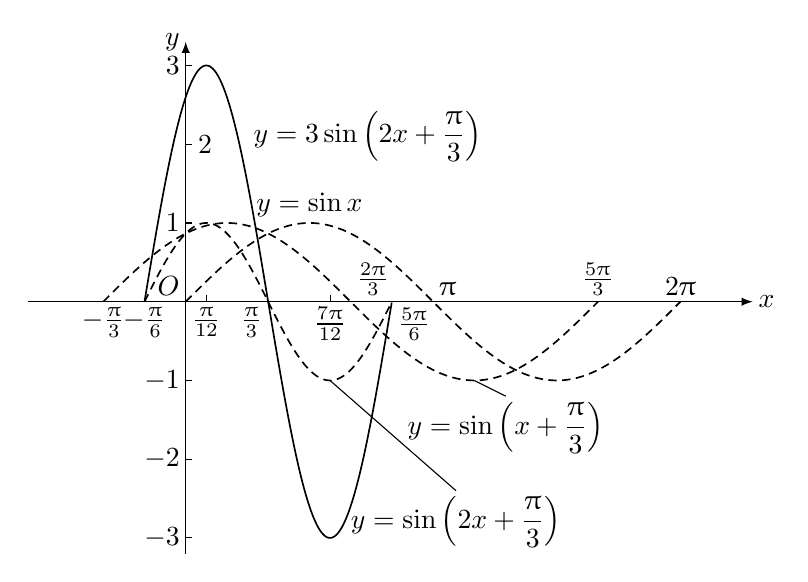
\begin{tikzpicture}[>=latex,scale=1.0,inner sep=2pt]
  \draw[->](-2,0)--(7.2,0)node[right]{$x$};
  \draw[->](0,-3.2)--(0,3.3)node[left]{$y$};
  \node at (0,0)[above left]{$O$};
  \draw[semithick,densely dashed,samples=200,domain=0:2*pi]plot(\x,{sin(\x r)});
  \draw[semithick,samples=200,domain=0:pi]plot(\x-pi/6,{3*sin(2*\x r)});
  \draw[semithick,densely dashed,samples=200,domain=0:pi]plot(\x-pi/6,{sin(2*\x r)});
  \draw[semithick,densely dashed,samples=200,domain=0:2*pi]plot(\x-pi/3,{sin(\x r)});
  \foreach \x in {-3,-2,-1,1,3} {\draw(0,\x)node[left]{$\x$}--++(0.08,0);}
  \draw(0,2)--++(0.08,0)node[right]{$2$};
  \node at (-pi/3,0)[below]{$-\frac\uppi3$};
  \node at (pi/3,0)[below left]{$\frac\uppi3$};
  \node at (-pi/6,0)[below]{$-\frac\uppi6$};
  \node at (5*pi/6,0)[below right]{$\frac{5\uppi}6$};
  \node at (pi,0)[above right]{$\uppi$};
  \node at (2*pi,0)[above]{$2\uppi$};
  \node at (2*pi/3,0)[above right]{$\frac{2\uppi}3$};
  \node at (5*pi/3,0)[above]{$\frac{5\uppi}3$};
  \draw[very thin](pi/12,0)node[below]{$\frac\uppi{12}$}--++(0,0.08);
  \draw[very thin](7*pi/12,0)node[below]{$\frac{7\uppi}{12}$}--++(0,0.08);
  \node at (0.5*pi,1)[above]{$y=\sin x$};
  \draw (7*pi/6,-1)--++(0.4,-0.2)node[below]{$y=\sin\left(x+\dfrac\uppi3\right)$};
  \draw (7*pi/12,-1)--++(1.6,-1.4)node[below]{$y=\sin\left(2x+\dfrac\uppi3\right)$};
  \node at (pi/4,2.5)[below right]{$y=3\sin\left(2x+\dfrac\uppi3\right)$};
\end{tikzpicture}
\end{document}